\chapter{Formal Analysis using Alloy}%
\label{chap:Formal-Analysis-using-Alloy}%

\par This section presents the formal analysis and verification of the system. The analysis is done using the Alloy
language and the Alloy Analyzer tool. The analysis is focused on modeling the temporal evolution and development of a
internship.

\section{Alloy Model}%
\label{sec:Alloy-Model}%

\par Here is the Alloy model of the system:

\begin{lstlisting}[language=Alloy]
        //actors
        sig Student {
            uni : one University,
        }
        
        //company signature
        sig Company {
            
        }
         
        //university signature, carries the information about the blocked companies
        sig University {
            blocked: set Company
        }
        
        //internship signature, carries most of the information about the entire process
        sig Internship {
            var state: one Status,
            var applicants: set Student, //applicants are the students that have applied and will recieve the Interview questionnaire
            var selected_student: lone Student,
            company: one Company,
            questionnaire: one Interview,
            deadline: one Date,
            var responses: set Student, //students that have responded to the Interview questionnaire
            duration: one WorkPeriod,
            feedback: one Feedback
        }
        
        //work period of the internship
        sig WorkPeriod{
            start: one Date,
            end: one Date
        }
        //generic questionnaire
        abstract sig questionnaire{
            
        }
        //interview questionnaire for the selection phase
        sig Interview extends questionnaire{
            
        }
        
        //feedback questionnaire for when the internship is completed without being calcelled
        sig Feedback extends questionnaire{
            var compiled_by: lone Student
        }
        
        
        //dates 
        sig Date{
            comes_later_than: set Date
        }
        
        
        //statuses for internships
        abstract sig Status{
        
        }
        
        one sig Created, Open, Selecting, Ongoing, Completed, Interrupted, Terminated extends Status{
        
        }      
\end{lstlisting}

\par The signatures that extend Status are used to represent the evolution of a intenship with time. Their meaning is
as follows:

\begin{itemize}
    \item Created: The internship has just been created nothing has happened yet.
    \item Open: The internship is open and students can now Apply.
    \item Selecting: The students recieved the Interview questionnaire and the company waits for their responses.
    \item Ongoing: The internship is ongoing and the selected student is working.
    \item Completed: The internship has been completed and the feedback has been compiled.
    \item Interrupted: Some problem has arisen and the internship has been interrupted.
    \item Terminated: Due to the problems previoulsy arisen the internship has been terminated. %(Bad Ending)
\end{itemize}

\par Facts of the model:

\begin{lstlisting}[language=Alloy]
                  
        //the student can't apply to internship if the company is blocked by the university
        fact blocked{
                all i: Internship | all st :i.applicants | i.company not in st.uni.blocked
            }
        
        //the work period starts later than the deadline
        fact breathing_room{
        all i: Internship | later_date[i.duration.start, i.deadline]
        }
        
        //the work period ends later than the start
        fact work_period_start_before_end {
        all wp: WorkPeriod | later_date[wp.end, wp.start]
        }
        
        //each internhips is offered by one company
        fact one_company_per_internship{
        all c1,c2 :Company | (c1 != c2) implies c1.company_internships & c2.company_internships = none
        }
        
        //total ordering on dates
        fact antisymmetry{
                all d1,d2:Date |  d1 in d2.comes_later_than  implies d2 not in d1.comes_later_than
            }
        fact transitivity{
                all d1,d2,d3 :Date | (d1 in d2.comes_later_than and d2 in d3.comes_later_than) implies d1 in d3.comes_later_than
            }
        fact  total_order{
        all  d1, d2 : Date |d1 != d2 implies  ( d1 in d2.comes_later_than or d2  in d1.comes_later_than)
        }
        fact no_reflexivity{
        all d:Date | d not in d.comes_later_than
        }
        
\end{lstlisting}

\par Facts that model the evulution of the internship:

\begin{lstlisting}[language=Alloy]
        //forces the initial state of every intership to be "Created"
        fact begin{
                always some i: Internship | i.state != Created implies once i.state = Created
            }
        
        //temporal evolution of the internship state
        //states represent a snapshot of the intersnhip right before the transition to the next state
        fact evolution{
                always all i:Internship | i.state = Created implies  i.state' = Open
                always all i:Internship | i.state = Open implies  i.state' = Selecting
                always all i:Internship | i.state = Selecting implies  i.state' = Ongoing
                always all i:Internship | i.state = Ongoing implies (i.state' = Completed or i.state' = Interrupted)
                always all i:Internship | i.state = Completed  implies i.state' = Completed
                always all i:Internship | i.state = Interrupted  implies (i.state' = Terminated or i.state' = Ongoing)
                always all i:Internship | i.state = Terminated  implies i.state' = Terminated
            }
\end{lstlisting}

\par This two facts model the internship transitions like a Finite State Machine. The machine is drawn here:

\begin{figure}[H]
    \centering
    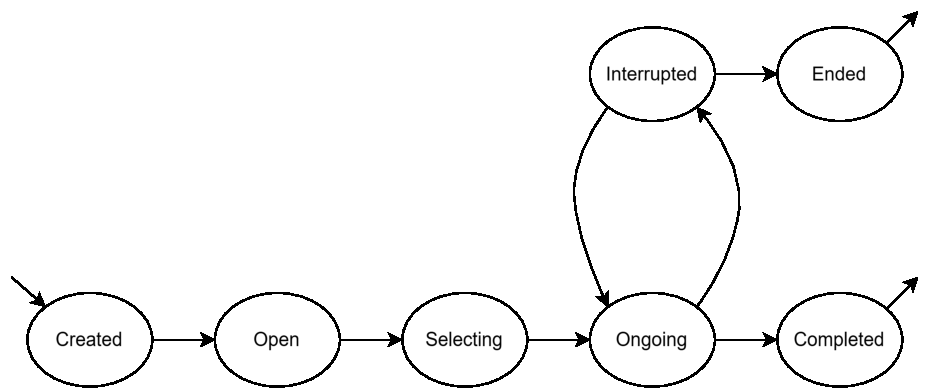
\includegraphics[width=0.6\textwidth]{Images/Alloy_images/FSM.pdf}
    \caption{Finite State Machine of the Internship}
\end{figure}

\begin{lstlisting}[language=Alloy]
        //initial state of the internship
        fact Created_is_uninitialized_state{
        always some i: Internship | i.state = Created implies (i.applicants = none and i.selected_student = none and i.responses = none)
        }
        
        //possible values of variables in states
        fact Open_is_only_for_applying{
        always some i: Internship | i.state = Open implies (i.responses = none and i.selected_student = none and i.applicants != none)
        }
        fact Selecting_is_for_interviews{
        always some i: Internship | i.state = Selecting implies (i.responses != none and i.selected_student = none) //applicants will be none because of persistence
        }
        fact Ongoing_means_selected{
        always some i: Internship | i.state = Ongoing implies i.selected_student != none
        }
        
        //constraints to ensure that variables evolve correctly, at the correct time and no information is lost
        fact responders_are_applicants{
        always all i:Internship | i.responses in i.applicants
        }
        fact Apply_only_when_open{
        always all i:Internship | (i.state != Created ) implies i.applicants = i.applicants' //the only transition that can change the applicants is the one from Created to Open
        }
        fact Respond_only_when_selecting{
        always all i:Internship | (i.state != Open ) implies i.responses = i.responses' //the only transition that can change the responses is the one from Open to Selecting
        }
        fact Select_only_before_Ongoing{
        always all i:Internship | (i.state != Selecting ) implies i.selected_student = i.selected_student' //the only transition that can change the selected_student is the one from Selecting to Ongoing
        }
        //in order to be selected the student must have responded to the interview questionnaire
        fact selected_has_responded{
        always all i: Internship | i.selected_student = none or i.selected_student in i.responses
        }
        
        //feedback is compiled only when the internship is completed
        fact uncompiled_feedback{
        always all i: Internship | i.state != Completed implies i.feedback.compiled_by = none
        }
        
        //if the internship is completed, the feedback must be compiled by someone
        fact feedback_compilation{
        all i: Internship | eventually i.state = Completed implies eventually i.feedback.compiled_by != none
        }
        
        //feedback is compiled by the selected student or by none if the internship is not completed
        fact compiled_by_selected{
        always all i: Internship | i.feedback.compiled_by = i.selected_student or i.feedback.compiled_by = none
        }
\end{lstlisting}

Useful assertions, predicates and functions used in the model itself and for testing it during the development:

\begin{lstlisting}[language=Alloy]
    
        //d1 is later than d2
        pred later_date[d1,d2: Date]{
        d2 in d1.comes_later_than
        }
        
        //does the university have multiple students?
        pred multiple_students[un:University]{
        #un.University_students > 1
        }
        
        //does the intenship terminate correctly?
        pred normal_development[i:Internship]{
        eventually i.state = Completed
        }
        
        //has the internship been interrupted?
        pred interrupted[i:Internship]{
                eventually i.state = Interrupted
            }
        
        //check the total number of applications recieved
        assert response_cardinality{
        always all i: Internship | #i.applicants >= #i.responses
        }
        
        //check for non emptiness
        assert ongoing_check{
        all i: Internship | i.state = Ongoing implies i.applicants != none and i.responses != none
        }
        
        //no internships gets stuck without a way to progress
        assert process_end{
        eventually all i: Internship | i.state = Completed or i.state = Terminated
        }
        
        //check for valid applicants (students that are not blocked by the company)
        assert valid_applicants{
        all i: Internship | all a: i.applicants | a in Student and i.company not in a.uni.blocked
        }
        
        //check for valid responses (students that are not blocked by the company)
        assert valid_responses{
        all i: Internship | all r: i.responses | r in i.applicants and r in Student and i.company not in r.uni.blocked
        }
        //returns the students of a university
        fun University_students[u:University] : set Student {
                {s:Student | s.uni = u}
            }
        //returns the internships of a company
        fun company_internships[c:Company] : set Internship {
                {i:Internship | i.company = c}
            }
        
\end{lstlisting}

\par In order to visualize the final model and to check that the behavior is consistent with the requirements, the
following predicates are used to generate instances:

\begin{lstlisting}[language= Alloy]
    //show an instanc where the isternship is completed
    pred show_Comp[i:Internship]{
        some i: Internship | eventually i.state = Completed and eventually #i.applicants > 1
    }
    //show an instance where the internship is interrupted and Terminates bocause of problematics
    pred show_Int[i:Internship]{
        some i: Internship | eventually i.state = Terminated and eventually #i.applicants > 1
    }
    //show an instance where the internship is interrupted and resumes an in the end is completed
    pred resume_after_Int[i:Internship]{
        some i: Internship | eventually i.state = Interrupted and  eventually i.state =Completed and eventually #i.applicants > 1
    }
\end{lstlisting}

\par It is important to note that the clause "\#i.applicants > 1" isn't necessary but it allows to generate more
interesting and meaningful instances.

\section{Alloy Results}%
\label{sec:Alloy-Results}%

\par The model has been tested using the Alloy Analyzer tool. The results are consistent with the requirements and the
model is correct.

\par Here are the results generated by running the show\_Comp predicate:

\par Created State:

\begin{figure}[H]
    \centering
    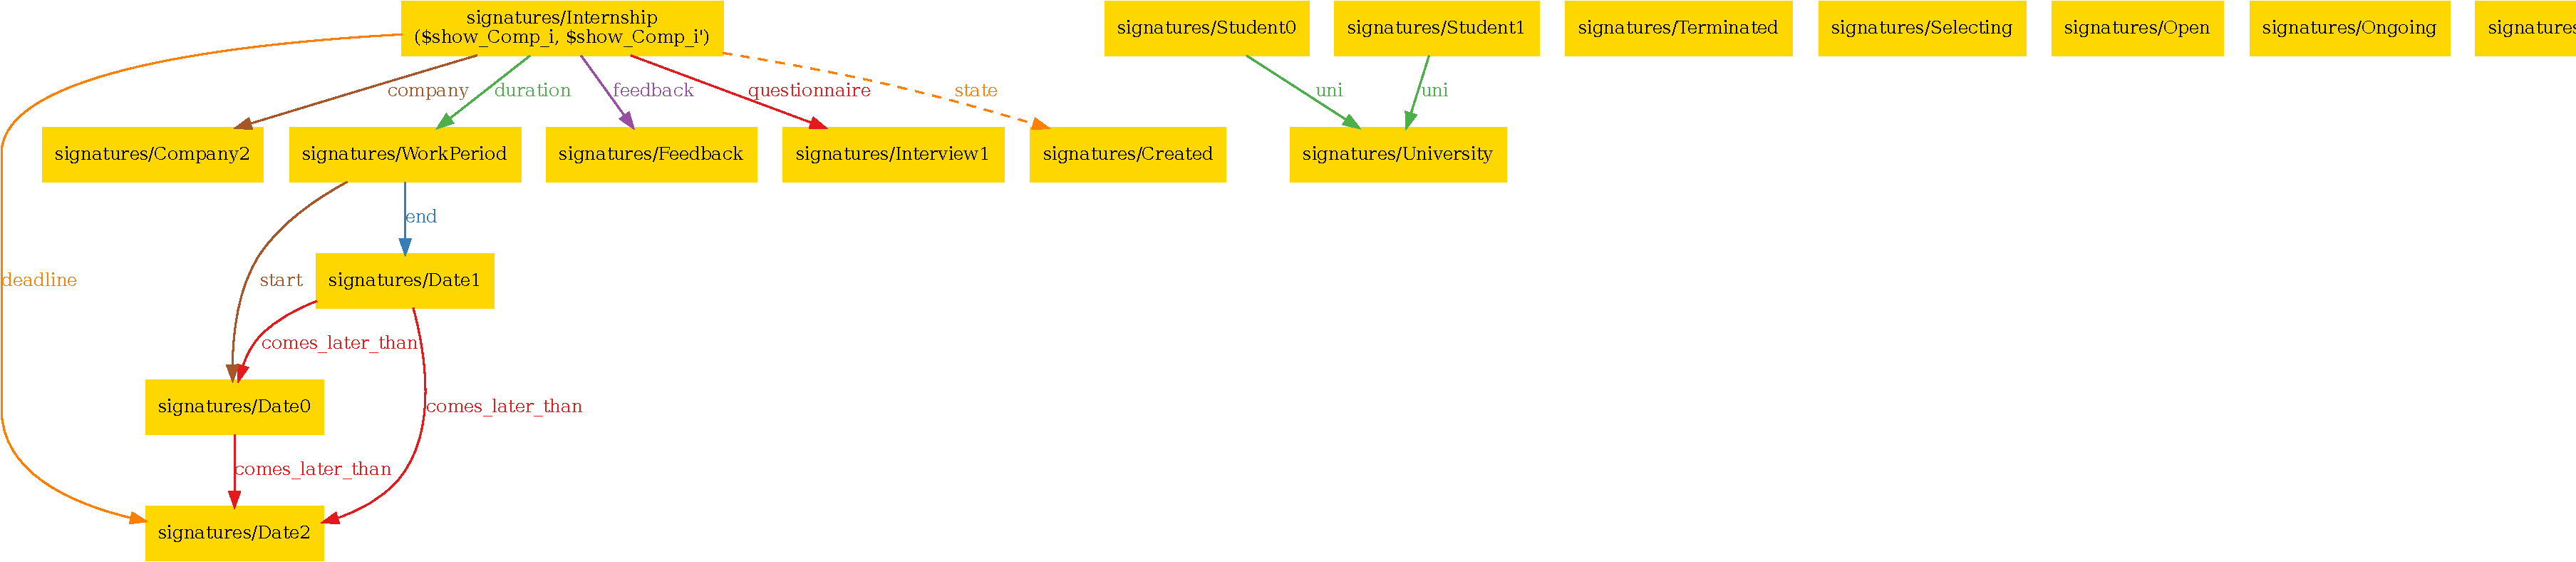
\includegraphics[width=1\textwidth,height=0.3\textheight]{Images/Alloy_images/Alloy_1-1.pdf}
    \caption{Created State}
\end{figure}

\par Open State:
\begin{figure}[H]
    \centering
    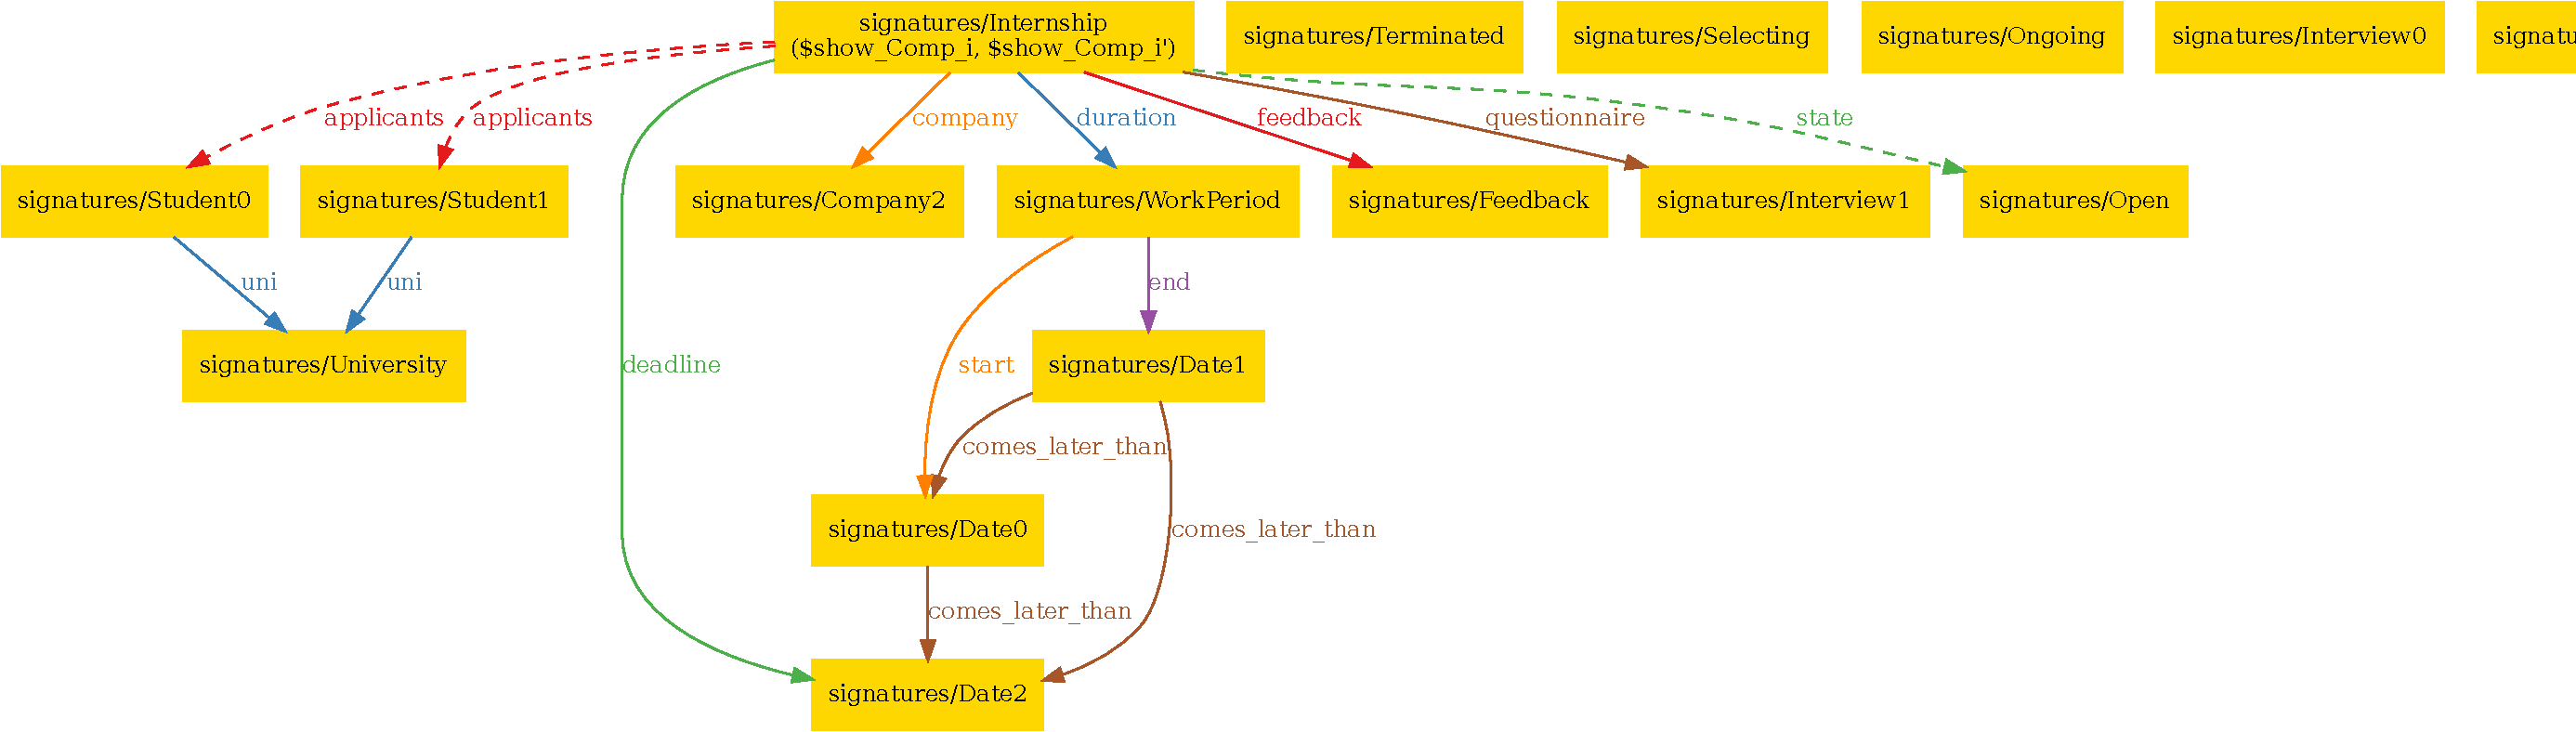
\includegraphics[width=1\textwidth,height=0.3\textheight]{Images/Alloy_images/Alloy_1-2.pdf}
    \caption{Open State}
\end{figure}

\par Selecting State:
\begin{figure}[H]
    \centering
    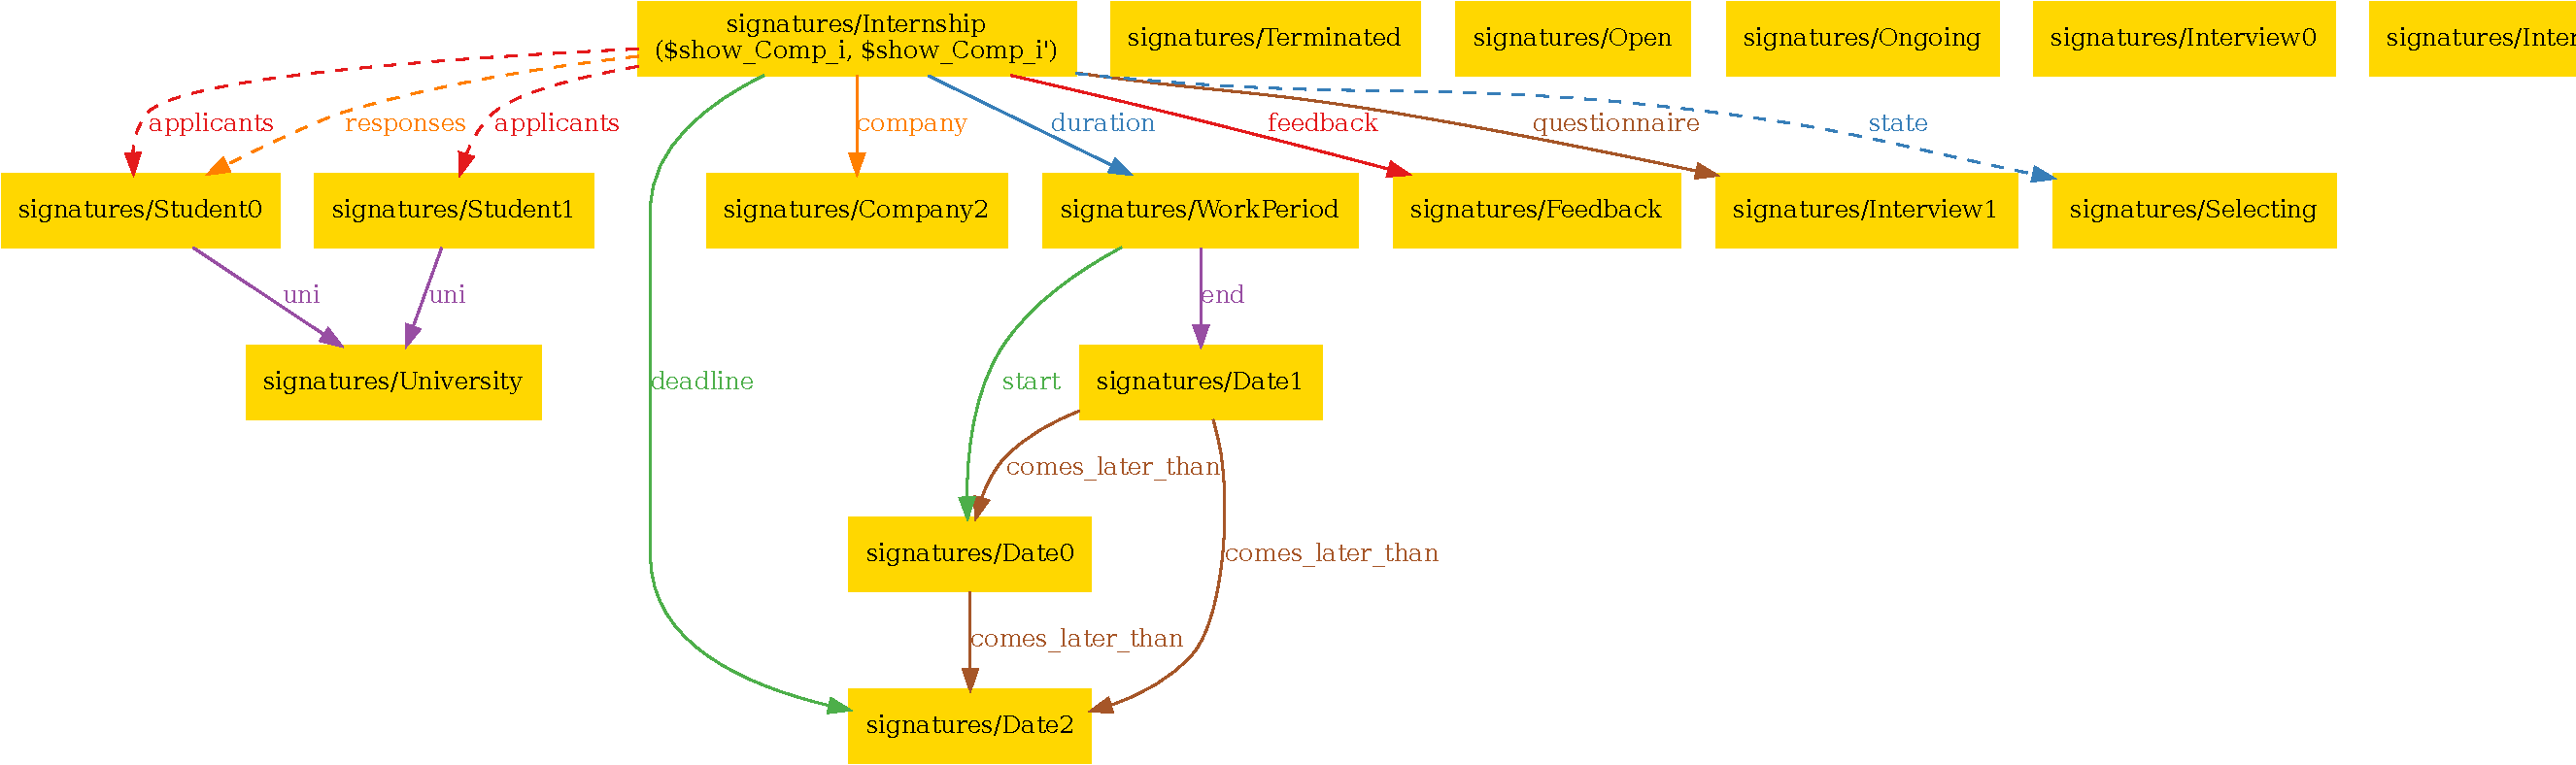
\includegraphics[width=1\textwidth,height=0.3\textheight]{Images/Alloy_images/Alloy_1-3.pdf}
    \caption{Selecting State}
\end{figure}

\par Ongoing State:
\begin{figure}[H]
    \centering
    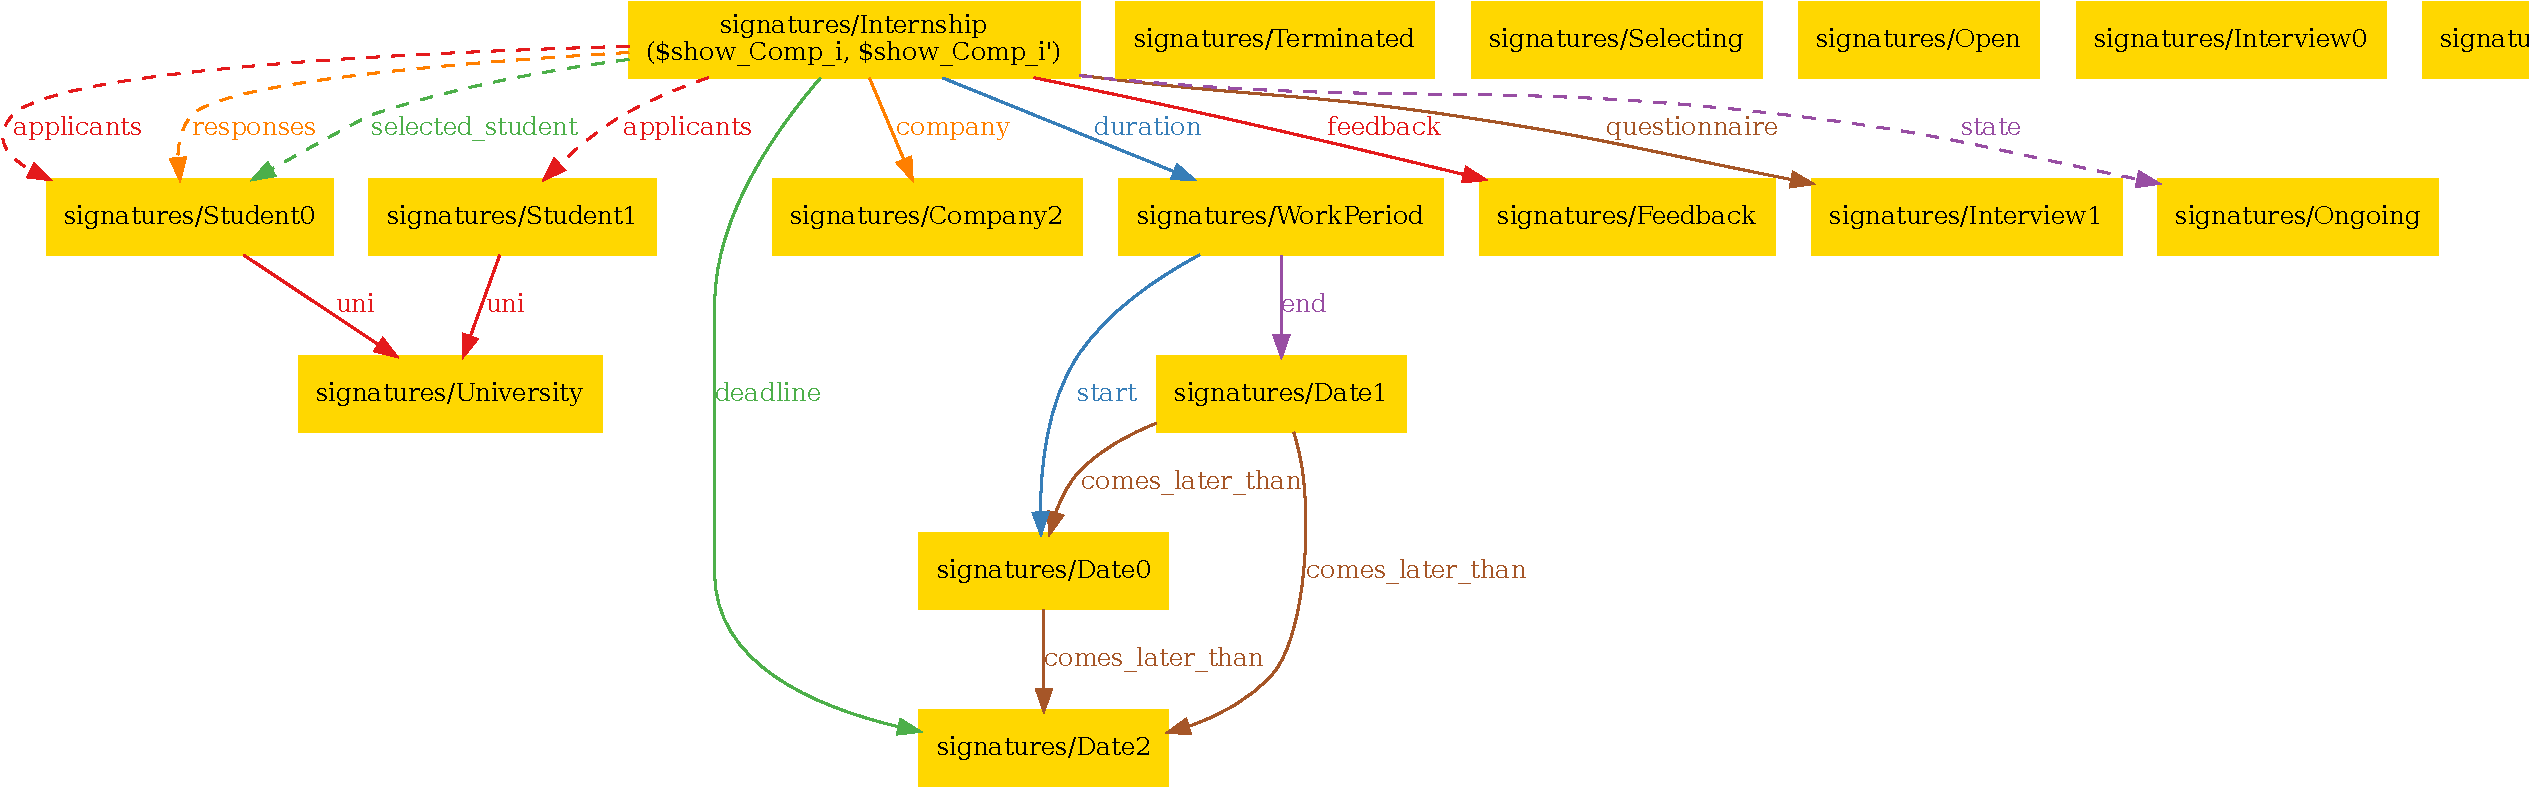
\includegraphics[width=1\textwidth,height=0.3\textheight]{Images/Alloy_images/Alloy_1-4.pdf}
    \caption{Ongoing State}
\end{figure}

\par Completed State:
\begin{figure}[H]
    \centering
    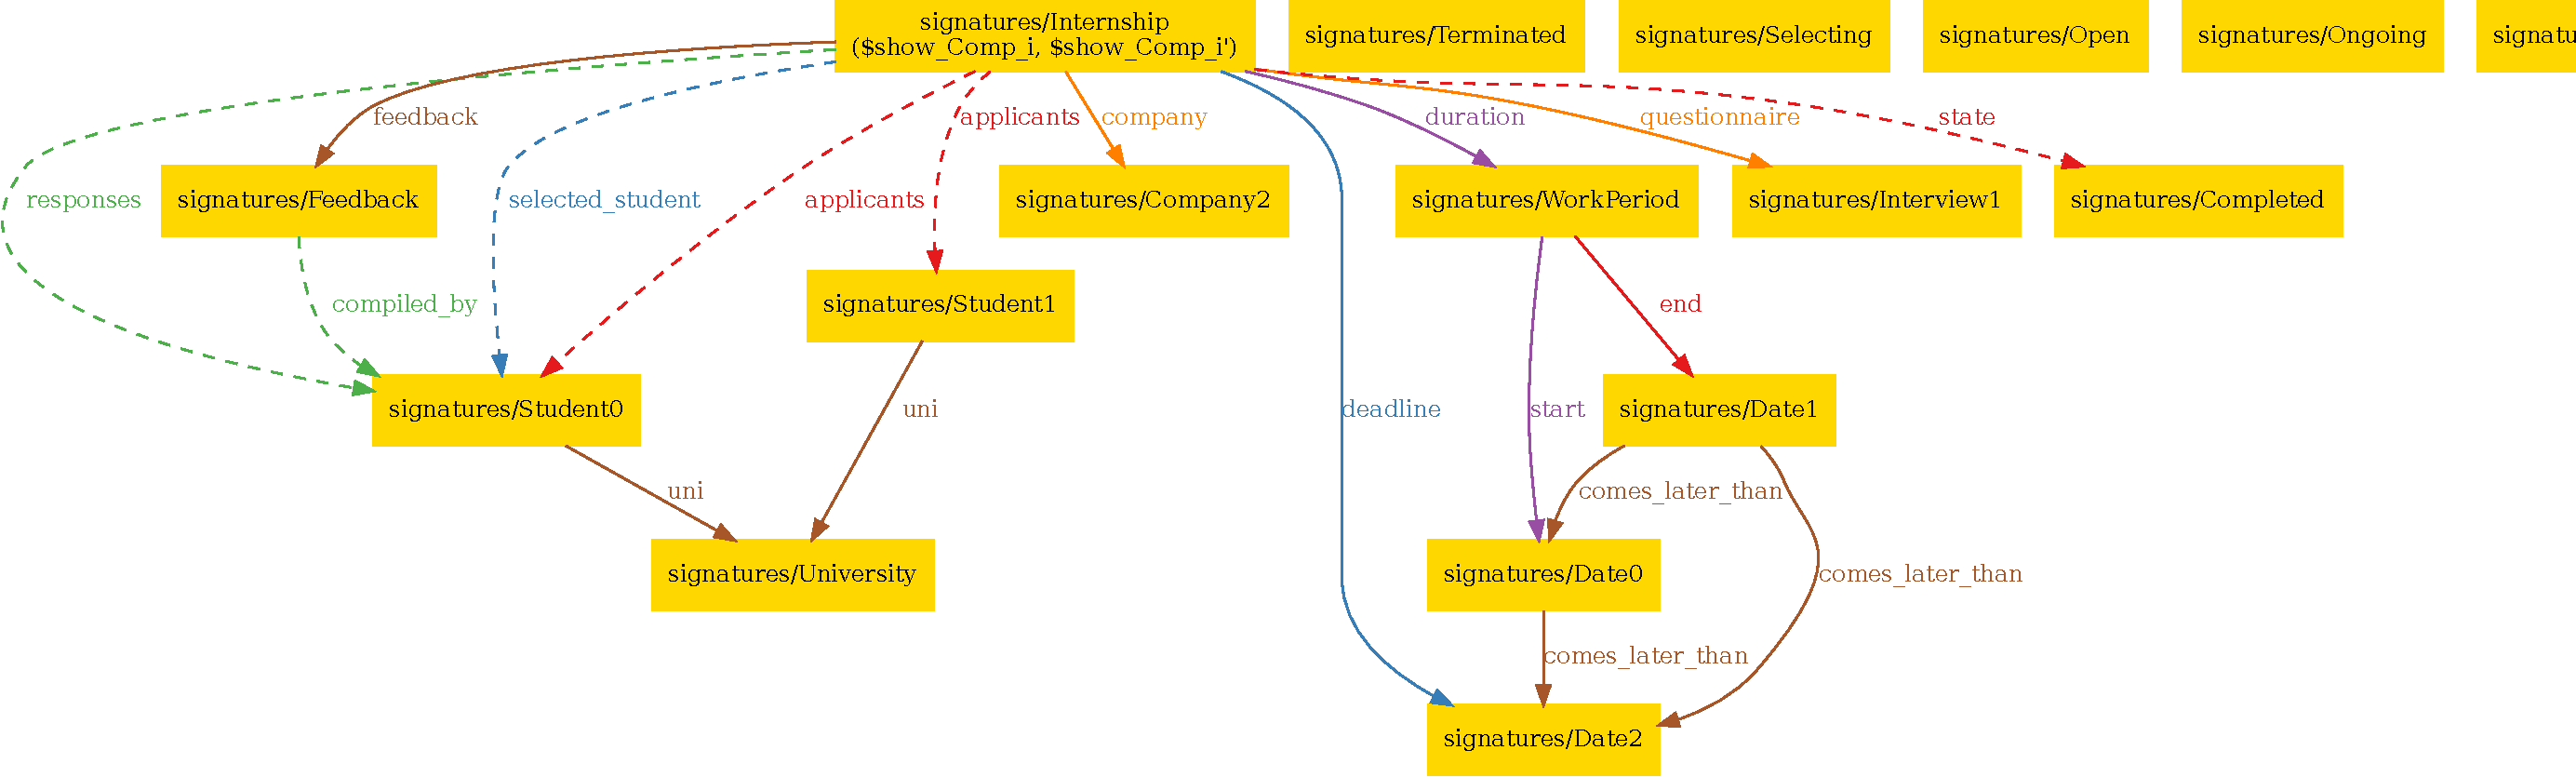
\includegraphics[width=1\textwidth,height=0.3\textheight]{Images/Alloy_images/Alloy_1-5.pdf}
    \caption{Completed State}
\end{figure}
